\section{Background estimation} \label{sec:bkg}

The largest background contributions from \Zvvjets~and \Wlvjets~processes
are estimated using data from four mutually exclusive control samples selected 
from dimuon, dielectron, single-muon, and single-electron states, 
as explained below. 

The remaining backgrounds that contribute to the total event yield in the signal region
are much smaller than those from \Zvvjets~and \Wlvjets~processes. These backgrounds
include QCD multijet events which are measured from data using a $\Delta\phi$ extrapolation 
method~\cite{Collaboration:2011ida,paper-exo-037}, and top-quark and diboson processes, which are 
obtained directly from simulation and are explained in the previous sections. 

\subsection{Signal extraction strategy}

A binned likelihood fit to the data (constructed as a product of poisson probabilities) as presented here:

\begingroup
\small
\begin{align}
\mathcal{L}(\boldsymbol{\mu}^{\Zvv}, \boldsymbol{\mu}, \boldsymbol{\theta}) = &
\prod_{i} \mathrm{Pois}\left(d_{i} | B_{i}(\boldsymbol{\theta}) + (1+f_{i}(\boldsymbol{\theta})_{\mathrm{QCD}}) \muz_{i} + R^{\mathrm{\Zvv}}_{i} (1+f_{i}(\boldsymbol{\theta})_{\mathrm{EW}}) \muz_{i}+ \boldsymbol{\mu} S_{i}(\boldsymbol{\theta})\right ) \times \nonumber\\
&\prod_{i} \mathrm{Pois} \left(d^{Z}_{i}|B^{Z}_{i}(\boldsymbol{\theta}) +\frac{\muz_{i} }{R^{Z}_{i} (\boldsymbol{\theta})_{\mathrm{QCD}}} + \frac{\muz_{i} }{R^{Z}_{i} (\boldsymbol{\theta})_{\mathrm{EW}}} \right) \nonumber\\
& \prod_{i} \mathrm{Pois}\left(d^{W}_{i}|B^{W}_{i}(\boldsymbol{\theta}) +\frac{f_{i}(\boldsymbol{\theta})_{\mathrm{QCD}}\,\muz_{i}}{R^{W}_{i}(\boldsymbol{\theta})_{\mathrm{QCD}}}+\frac{f_{i}(\boldsymbol{\theta})_{\mathrm{EW}}\,\muz_{i} }{R^{W}_{i} (\boldsymbol{\theta})_{\mathrm{EW}}} \right) \times \nonumber\\
\end{align}
\endgroup

The fit is performed simultaneously in the four different control samples and in the signal 
region, for events selected in the vbf category, to estimate the $\Zvvjets$ and $\Wlvjets$ rate
in each $m_{jj}$ bin. In this likelihood, the expected number of $\Zvvjets$ events in each 
bin of $m_{jj}$ are the free parameters of the fit. 
The $\Zvvjets$ and $\Wlvjets$ rates are estimated seperately for the 
QCD and EW components seperately in each $m_{jj}$ bin. However the fit is constrained using the $R^{\mathrm{\Zvv}}_{i}$ which 
demonstrates the ratio between the QCD and EW components of the $\Zvvjets$ background. This ratio does not have any additional 
uncertainty.
The systematic uncertainties ($\boldsymbol{\theta}$) 
enter the likelihood as additive perturbations to the transfer factors $R^{/Z/W}_{i}$, and are modeled as Gaussians.
The parameter $\boldsymbol{\mu}_{i}^{\Zvv}$ represents the yield of the $\Zvvjets$ background in the $i$ dijet mass 
bin into the signal region, and is left freely floating in the fit. The function $f_{i}(\boldsymbol{\theta})$ is the 
transfer factor between the $\Zvvjets$ and $\Wlvjets$ backgrounds in the signal region and represents a constraint between 
these backgrounds. The likelihood also includes the signal region  with $B_{i}$ representing all the backgrounds, $S$ 
representing the nominal signal prediction, and $\mu$ being the signal strength parameter also left floating in the fit. 

\subsection{Transfer factors}

Transfer factors, derived from simulation, 
are used to link the yields of the $\Zlljets$ and $\Wlvjets$ processes in the control
regions with the $\Zvvjets$ and $\Wlvjets$ background estimates in the signal region.
These transfer factors are defined as the ratio of expected yields of the target process
in the signal region and the process being measured in the control sample. As an example:
\begin{equation}
R_{i}^{Z} = \frac{N_{i,MC}^{\Zmm}}{N_{i,MC}^{\Zvv}} 
\end{equation}
where $N_{i}$ is the number of events in bin $i$ of the dijet mass distribution, $R_{i}$ is the transfer factor between the dimuon control region and $\Zvv$ background. 
Other transfer factors are constructed in similar manner. 

To estimate the \Wlvjets~background in the signal region, the transfer factors between
the \Wmvjets~and \Wevjets~event yields in the single-lepton control samples and
the \Wlvjets~ background estimates in the signal region are constructed. These transfer factors take into account 
the impact of lepton acceptances and efficiencies, lepton veto efficiencies, and
the difference in the trigger efficiencies in the case of the single-electron control sample. 
These transfer factors
are shown in Figure~\ref{fig:WMvvscalefactor}. The dotted red (blue) line shows the ratio of the processes where the V-boson
is produced via EW (QCD) production where as the solid lines show the ratio of the processes where the V-boson is produced both
via EW and QCD production.


\begin{figure}[htbp]
  \centering
        
\includegraphics[width=0.45\textwidth]{placeholder.png}   
        
\includegraphics[width=0.45\textwidth]{placeholder.png} 
  \caption{Transfer factors for the \Wlv background as a function of the dijet mass using the single muon and single electron control regions for the vbf final state. The grey band shows the statistical and systematic uncertainties on the ratios.}
    \label{fig:WMvvscalefactor}
\end{figure}


The \Zvv~background prediction in the signal region is connected to the yields of \Zmm~and \Zee~events
in the dilepton control samples. The associated transfer factors account for the differences in the
branching ratio of Z bosons to charged leptons relative to neutrinos and and the impact of lepton acceptance and selection 
efficiencies. In the case of dielectron events, the transfer factor also takes into account the 
difference in the trigger efficiencies. The resulting constraint on the \Zvv~background from the dilepton
control samples is limited by the statistical uncertainty in the dilepton control samples due to the large
branching fraction difference of the Z boson decays to muons and electrons compared to that to neutrinos.
These transfer factors are shown in Figure~\ref{fig:ZvvZmmSF}. The dotted red (blue) line shows the ratio of the processes where the V-boson
is produced via EW (QCD) production where as the solid lines show the ratio of the processes where the V-boson is produced both
via EW and QCD production.

\begin{figure}[htbp]
  \centering
        
\includegraphics[width=0.45\textwidth]{placeholder.png}
        
\includegraphics[width=0.45\textwidth]{placeholder.png}
\\
  \caption{Transfer factors for the \Zvvjets background as a function of the dijet mass using the dimuon, and dielectron control regions in vbf final state. The grey band shows the statistical and systematic uncertainties on the ratios. }
    \label{fig:ZvvZmmSF}
\end{figure}


Finally, a transfer factor is also defined to connect the \Zvvjets~and \Wlvjets~background yields 
in the signal region to further benefit from larger statistical power that \Wlvjets~background has
making it possible to experimentally constrain \Zvvjets~production at high dijet masses.
These transfer factors are shown in Figure~\ref{fig:WZ_SF_vbf}. The dotted red (blue) line shows the ratio of the processes where the V-boson
is produced via EW (QCD) production where as the solid lines show the ratio of the processes where the V-boson is produced both
via EW and QCD production.

\begin{figure}[htbp]
  \centering
  
\includegraphics[width=0.45\textwidth]{placeholder.png}
  \caption{Transfer factors for the to estimate the Z($\nu\nu$)+jets background from W+jets in the signal region as a function of the dijet mass for the vbf final state. The grey band shows the statistical and systematic uncertainties on the ratios.}
  \label{fig:WZ_SF_vbf}
\end{figure}

\subsection{Systematic uncertainties}

Systematic uncertainties in the transfer factors are 
modeled as constrained nuisance parameters and include both
experimental and theoretical uncertainties
in the \Wjets~to \Zjets~differential cross section ratios. 

\subsubsection{Theoretical uncertainties}

Theoretical uncertainties in V+jets processes include effects from QCD and EW higher-order
corrections along with PDF modeling uncertainty. One of the uncertainties considered comes from the 
variations around the central renormalization and factorization scale choice. It is evaluated by taking the differences in the NLO cross 
section as a function of boson \pt after changing the renormalization and factorization scales by a factor of two and a factor 
of one-half with respect to the default value. These constant scale variations mainly affect the 
overall normalization of the boson \pt distributions. This uncertainty is treated to be uncorrelated 
across the \Zjets, \Wjets~processes, but correlated across the bins of the dijet mass distribution. 

The PDF uncertainty has been estimated using the standard deviations of
weights provided in the NNPDF3.0 parton distribution set and 
using the RMS of each bin of the distribution after varying the full
spectra by these weights. This uncertainty is treated to be correlated across the 
\Zjets, \Wjets~processes, and the bins of the dijet mass distribution.

The uncertainty due the EW corrections is assumed to be the full correction itself as 
a conservative approach. The uncertainty is treated correlated across the processes and 
across the bins of the dijet mass spectra.

These uncertainties are applied to the QCD and EW V+jets processes, but are assumed to be uncorrelated. That is, the QCD \Wjets~component has a factorization scale uncertainty that is the same size as the factorization scale uncertainty on the EW \Wjets~component, but the two are treated as separate nuisances in the signal extraction fit.

The summary of the aforementioned theoretical uncertainties including their magnitude per process 
and on the ratio are shown in Figure~\ref{fig:theory_unc}

\begin{figure}[htb!]
  \begin{center}
    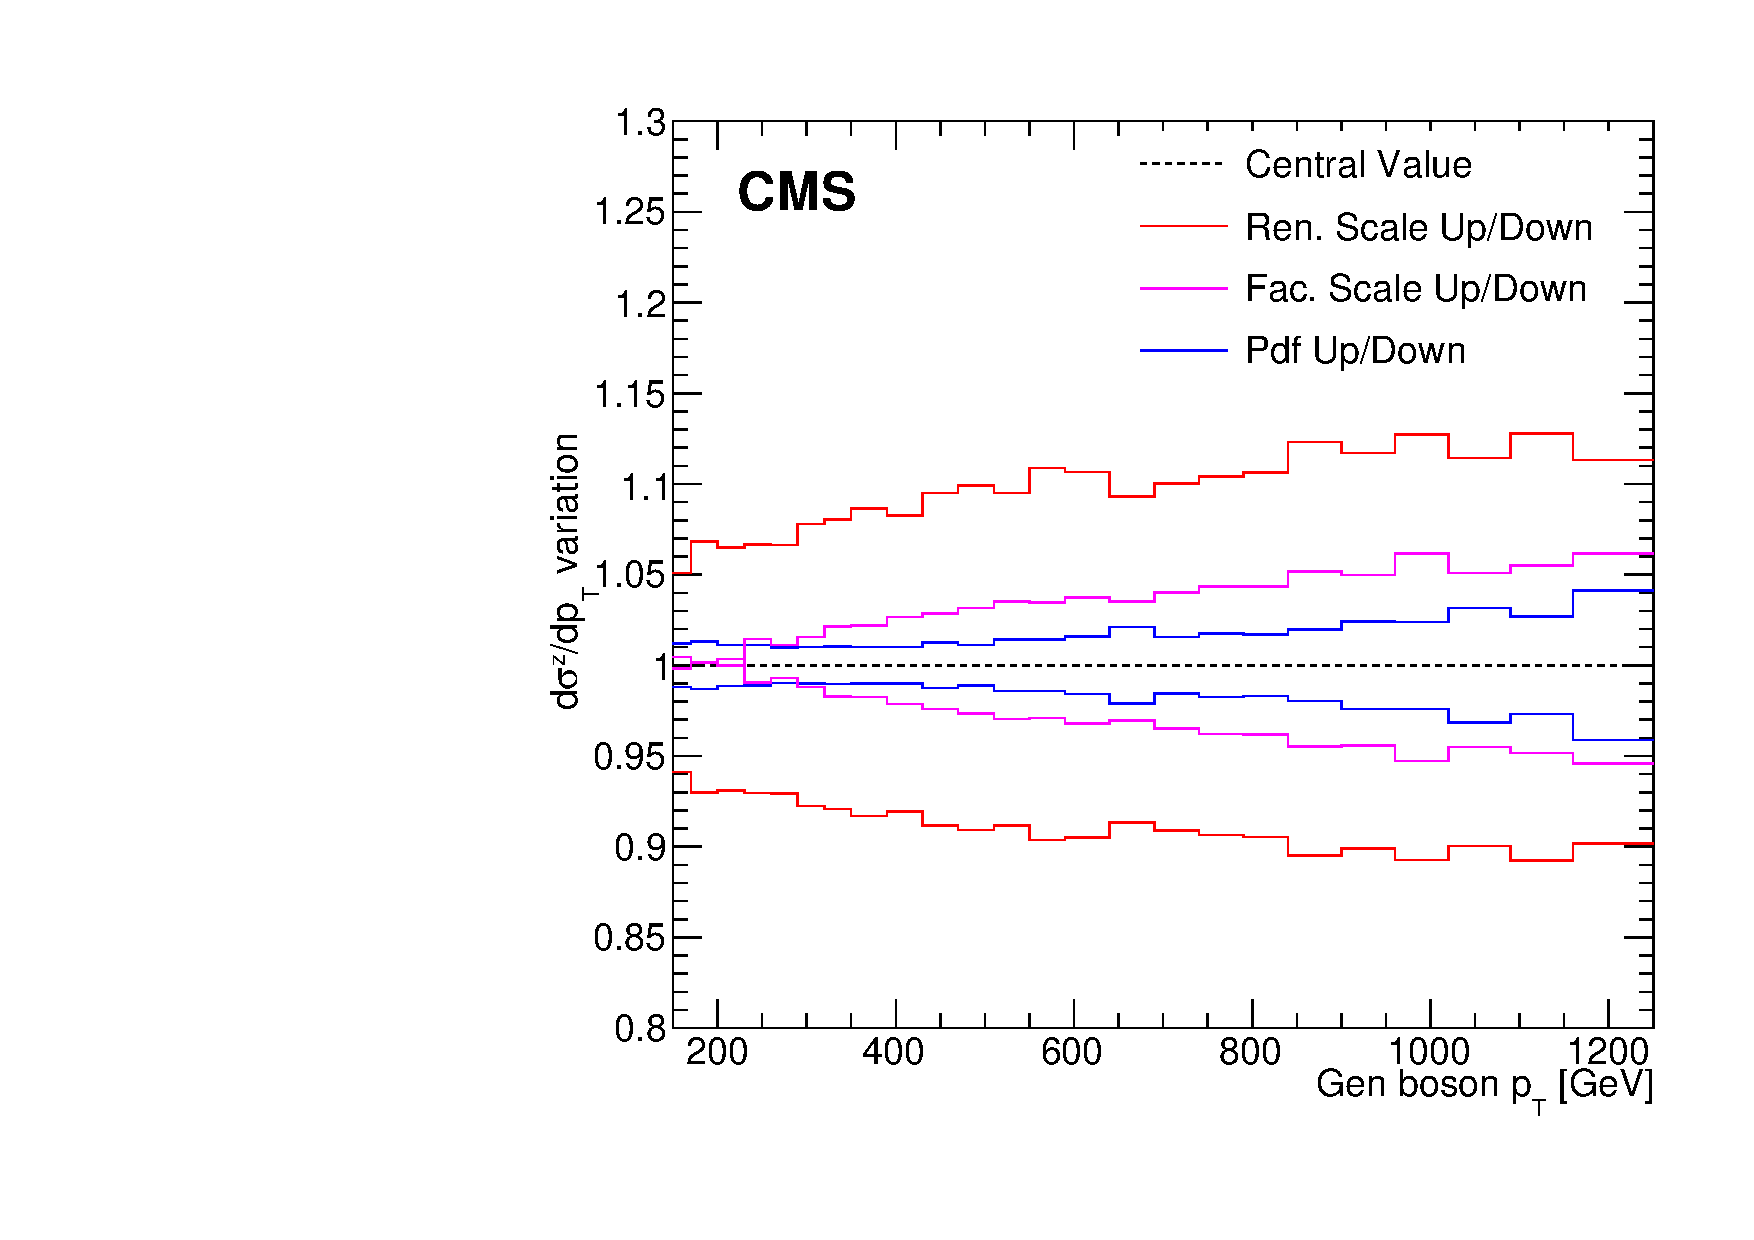
\includegraphics[width=0.48\textwidth]{fig/theory/zratio_unc.pdf}
    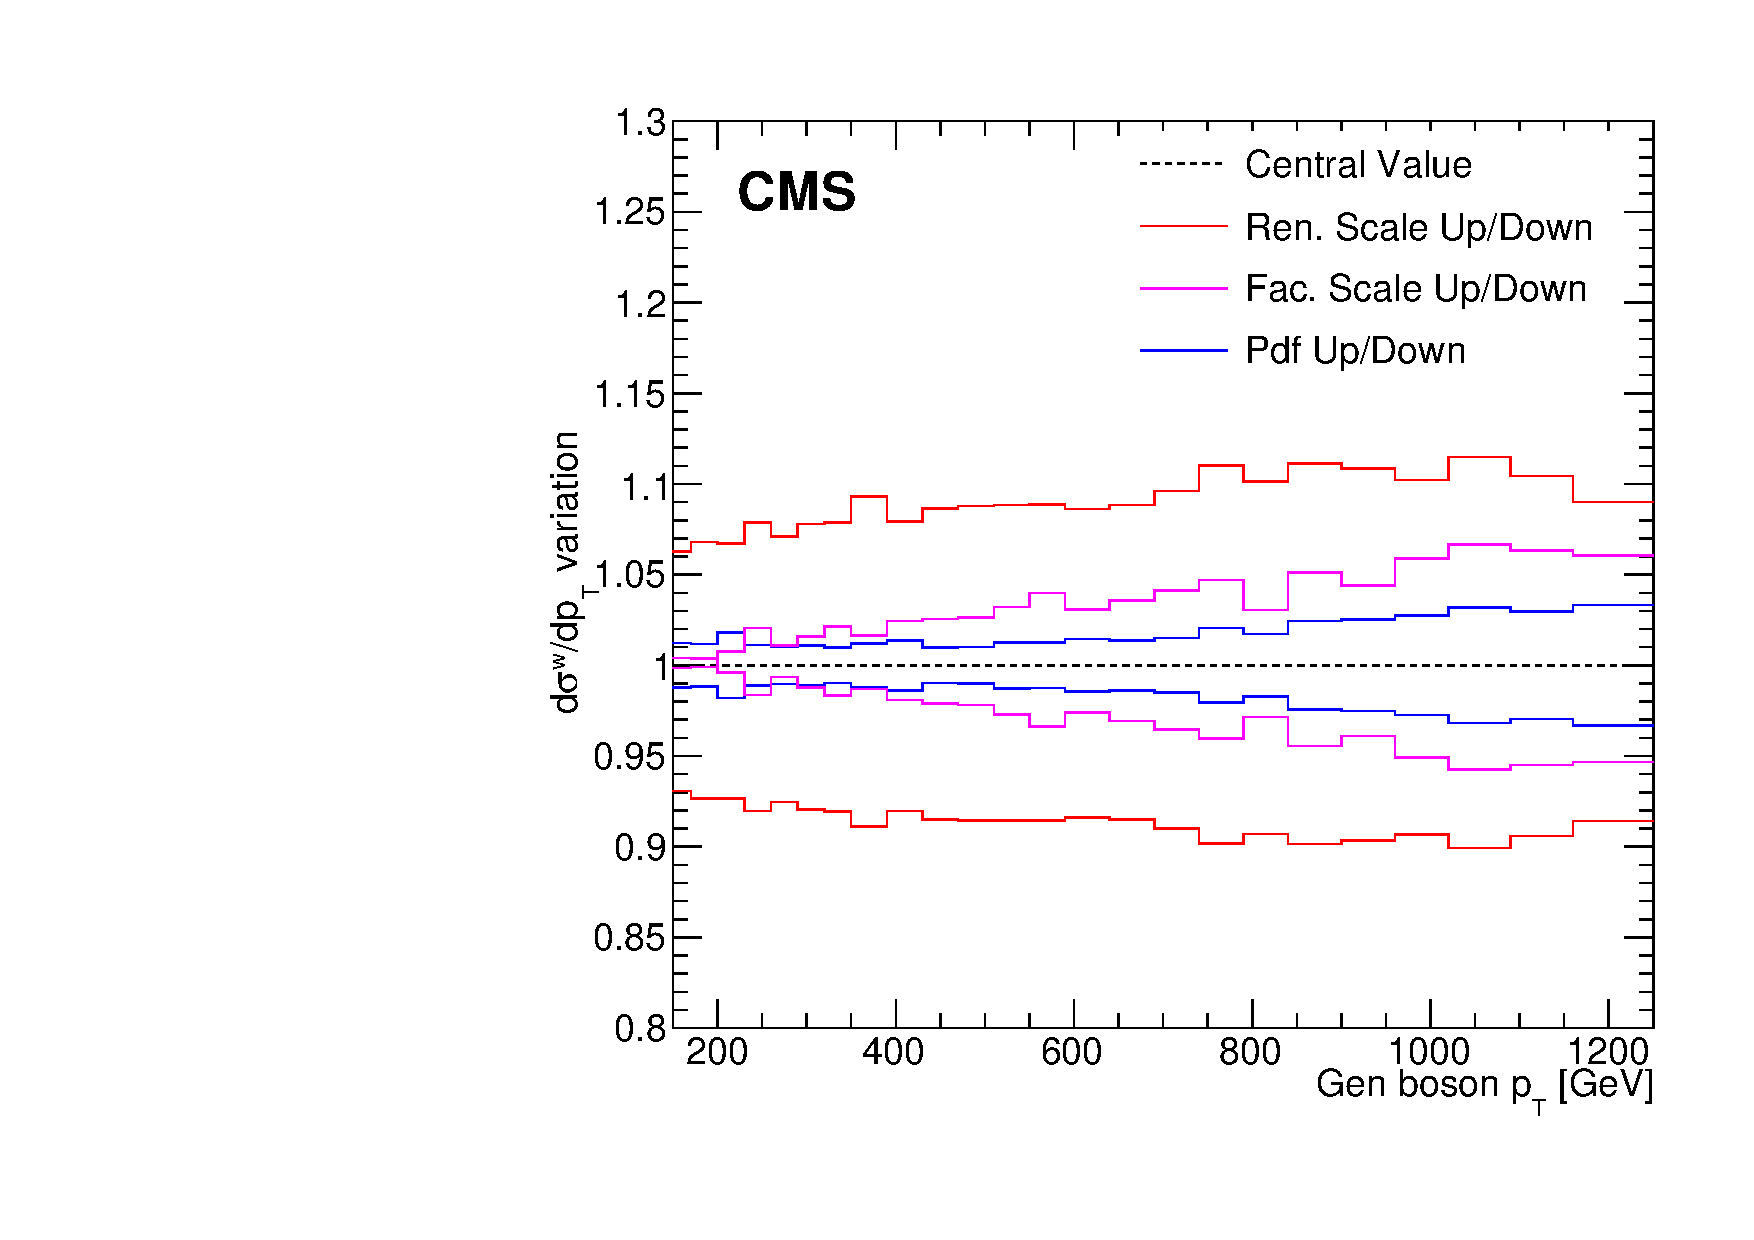
\includegraphics[width=0.48\textwidth]{fig/theory/wratio_unc.pdf}\\
    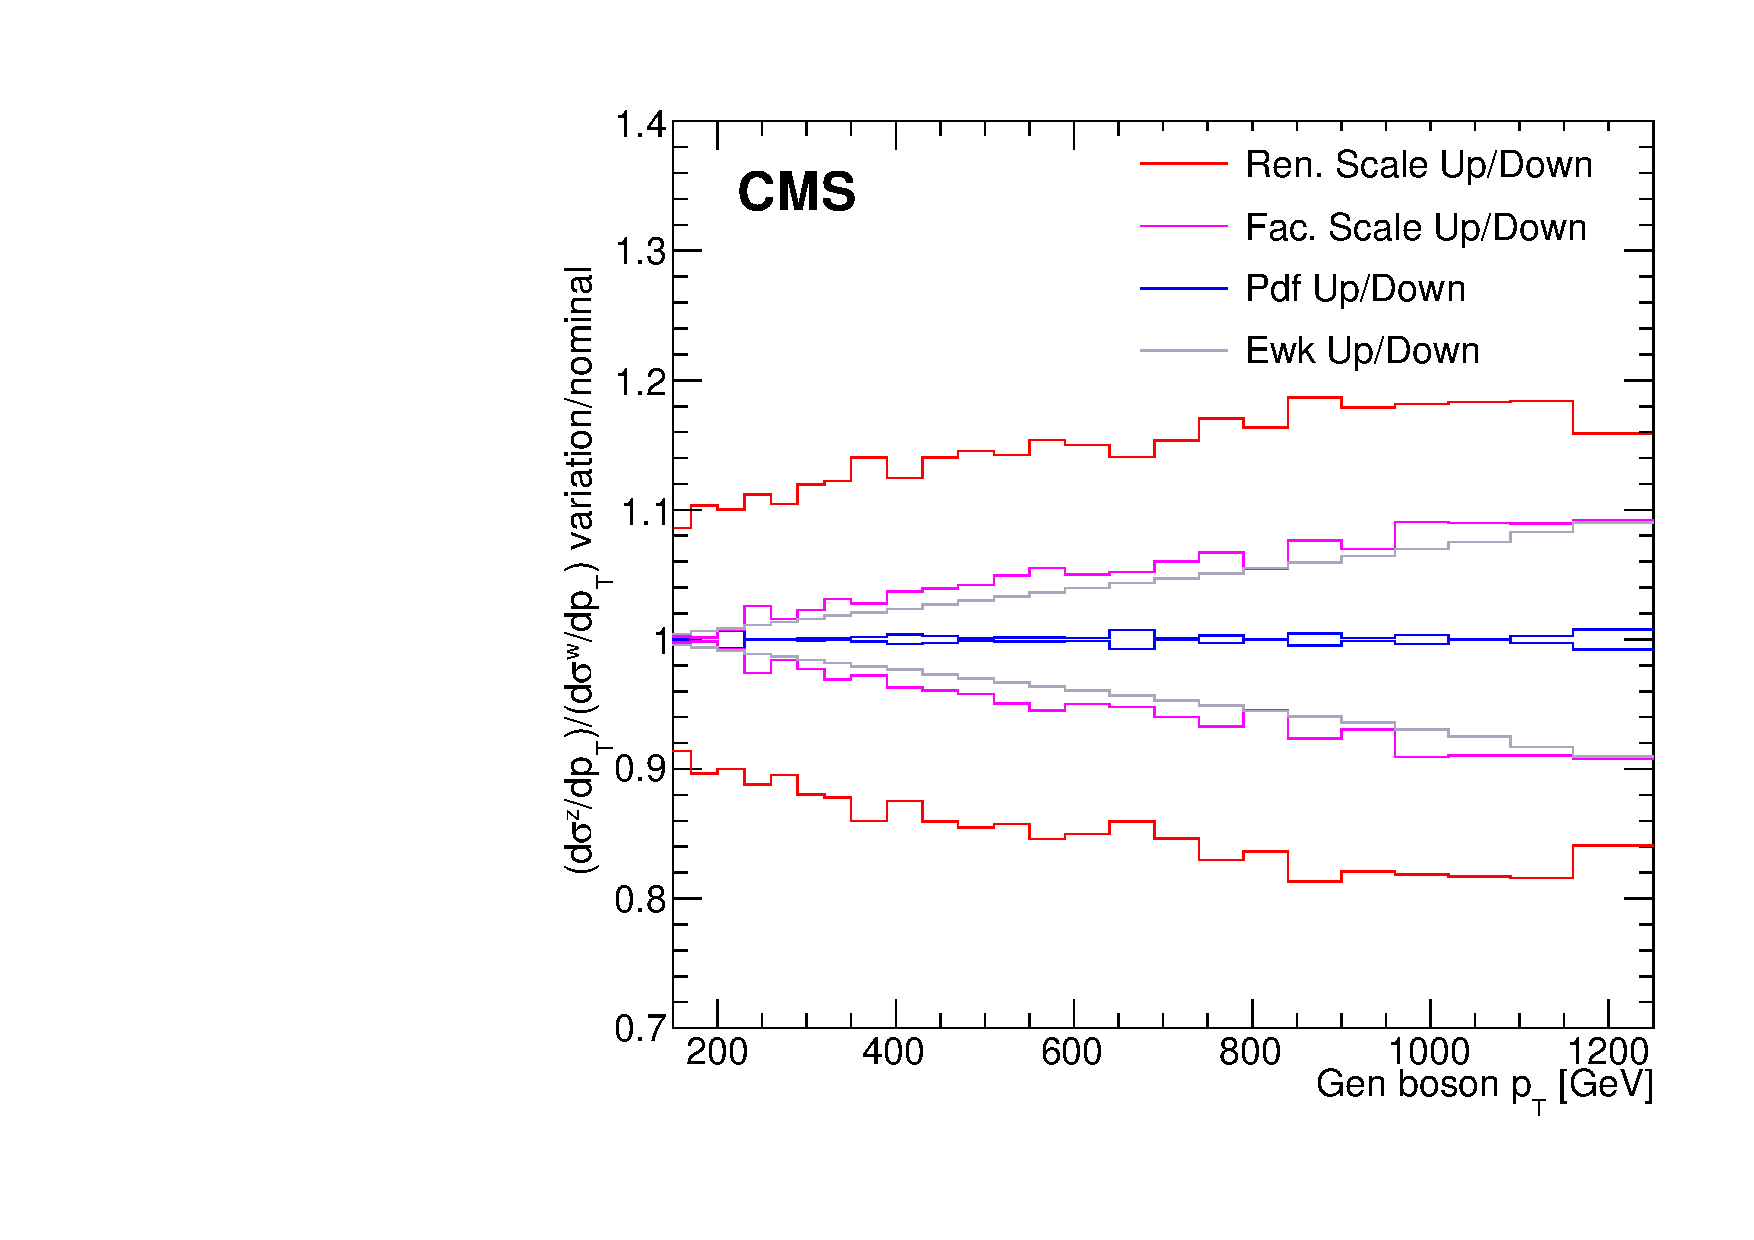
\includegraphics[width=0.48\textwidth]{fig/theory/bosonpt_ratio_uncertainty.pdf}
    \caption{Theoretical uncertainties due to QCD and EW higher-order corrections and the PDF variation is shown for individual processes and for the ratio.}
    \label{fig:theory_unc}        
  \end{center}                               
\end{figure}                                 

\subsubsection{Experimental uncertainties}
{\color{red} Check numbers for 2017/18}
Experimental uncertainties including the reconstruction efficiency 
(1\% per muon or electron), and selection efficiencies of leptons 
(1\% per muon and 2\% per electron), and hadronically 
decaying $\tau$ leptons (5\%) are incorporated to the analysis. 
These reconstruction and selection efficiencies further translate into an 
uncertainty in the lepton veto efficiency of 3\%. The lepton veto uncertainties in the transfer 
factors and are estimated through propagating the
overall uncertainty on the tagging scale factor (loose-muon ID, 
veto-electron ID and loose MVA-tau ID) into the vetoed selection 
based on both the flavour composition of the \Wjets~process the acceptance of the lepton. 
The overall magnitude of the lepton-veto uncertainty is found to be around 3~(4)\% 
and is found to be dominated by the $\tau$-veto uncertainty. 


The uncertainty in the modeling of \MET in simulation~\cite{Khachatryan:2014gga} 
is estimated to be 1-2\% on the ratios and is dominated by the uncertainty on the jet energy scale. The
jet energy scale uncertainties found to be not-cancelling in the ratio due to the differences in the 
jet kinematics between control and signal regions. The resulting jet energy scale uncertainties in the 
ratios can be seen in Figure~\ref{fig:unc_jec}

\begin{figure}[!htb]
\begin{center}
  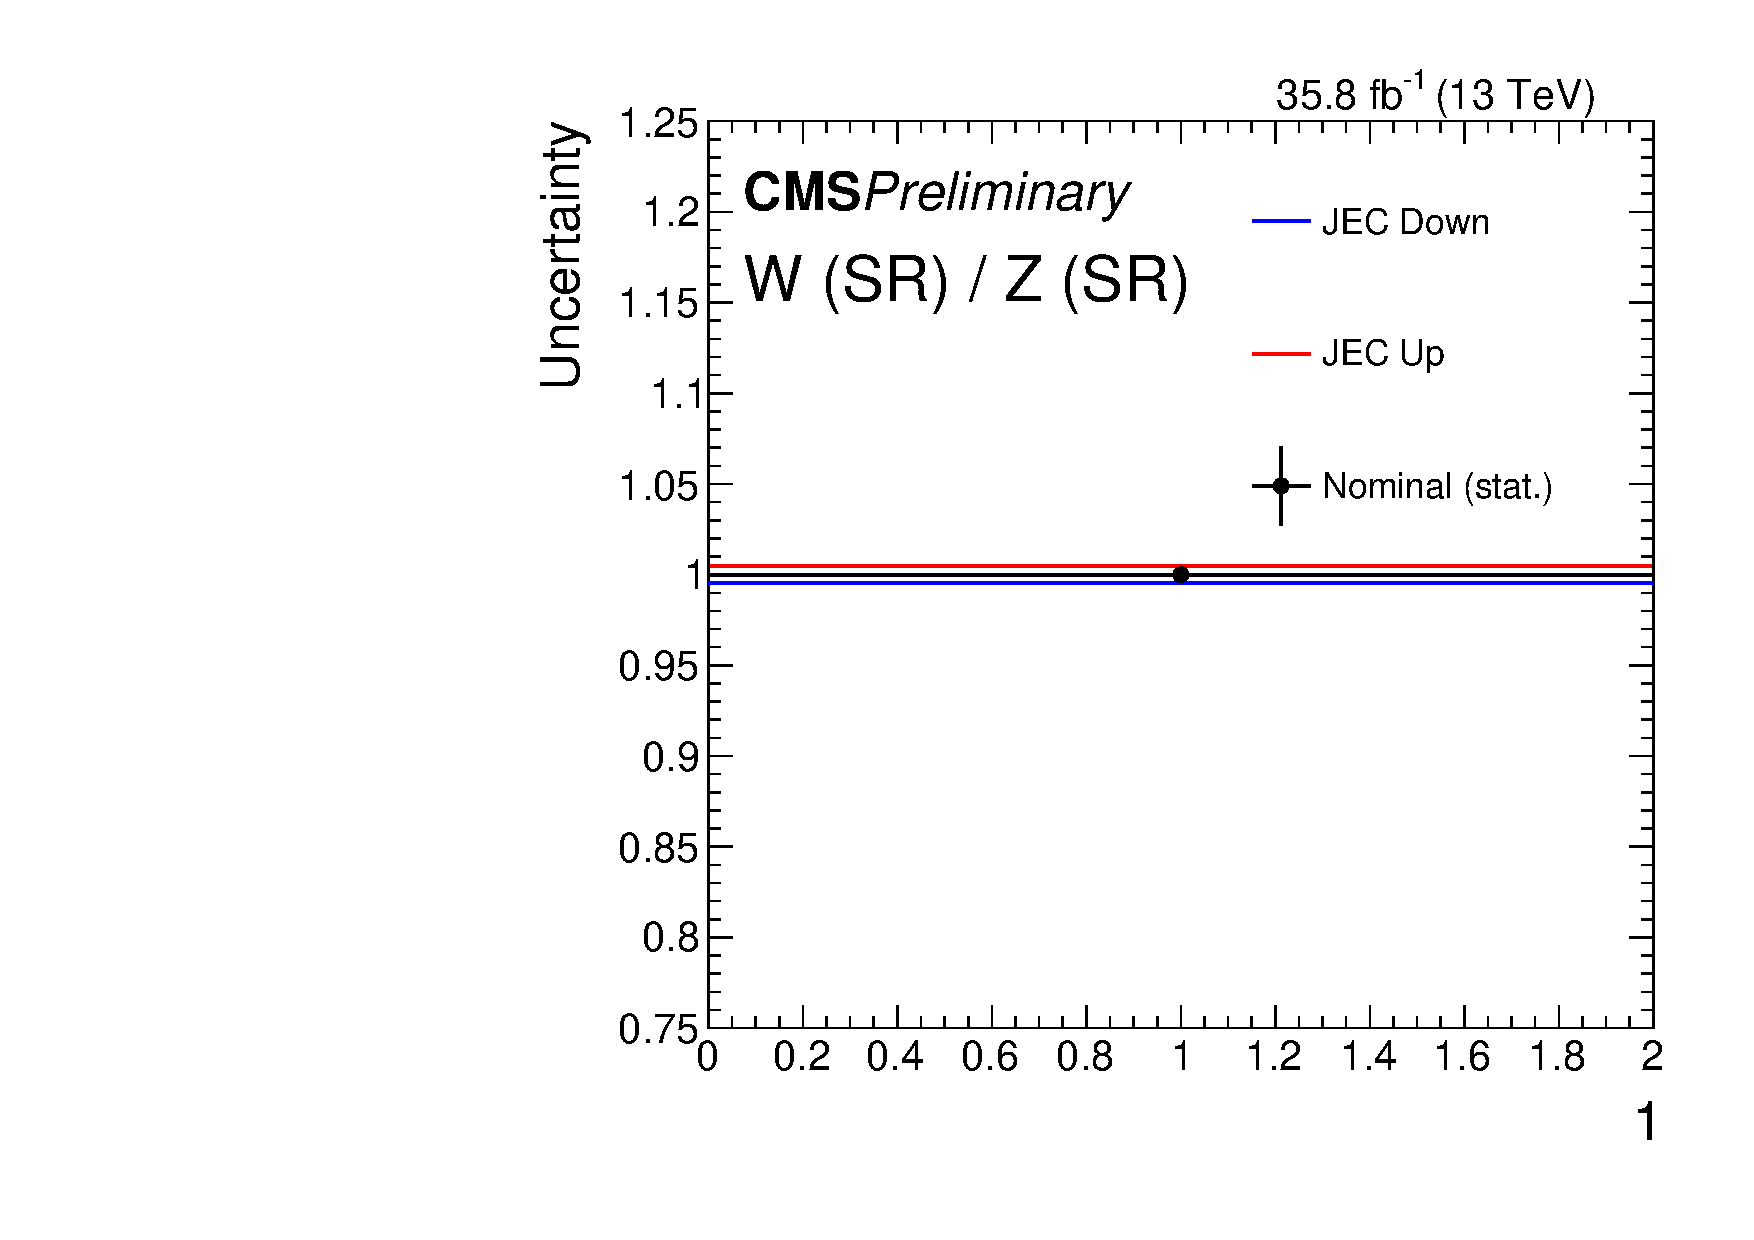
\includegraphics[width=0.45\textwidth]{fig/unc/jec_ratio_WJets_signal_signal_1.pdf}
  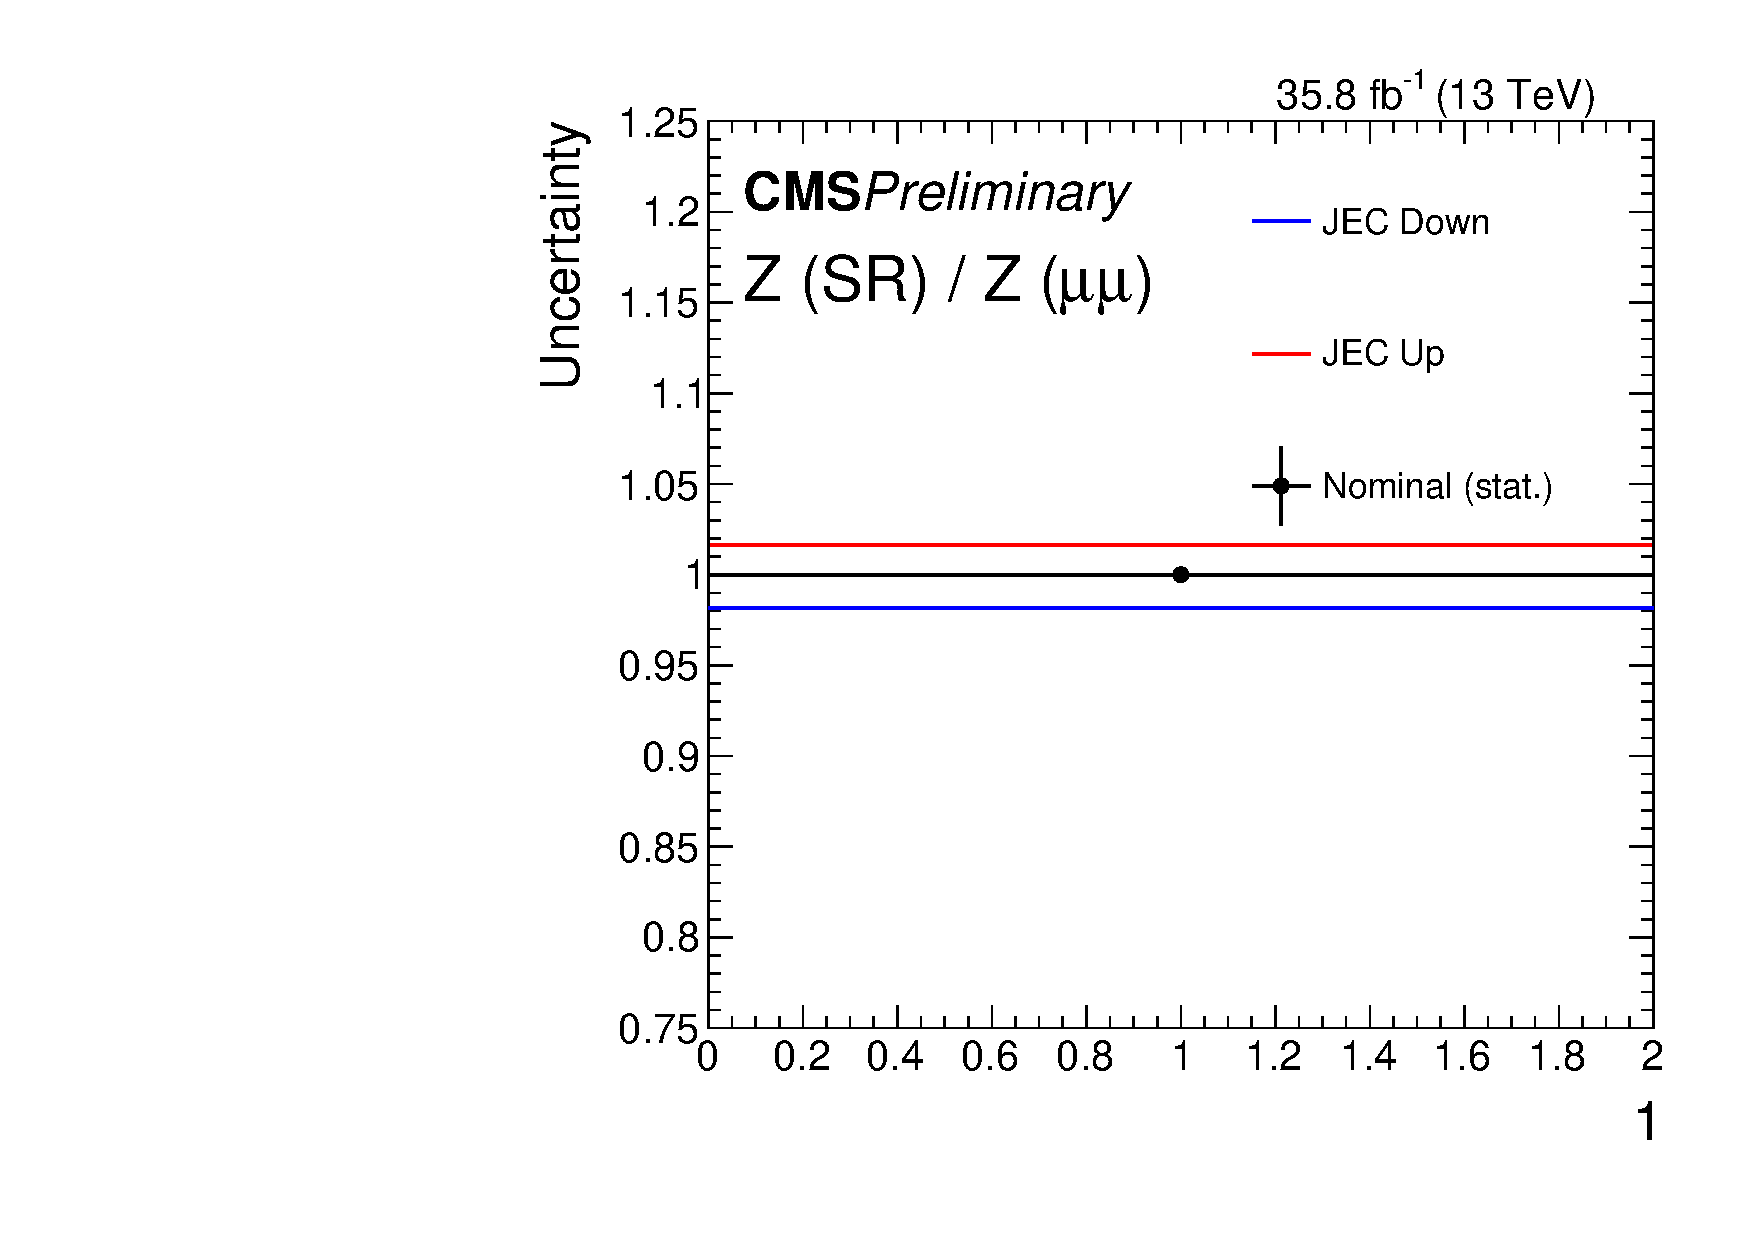
\includegraphics[width=0.45\textwidth]{fig/unc/jec_ratio_ZtoNuNu_signal_dimuon_1.pdf}
  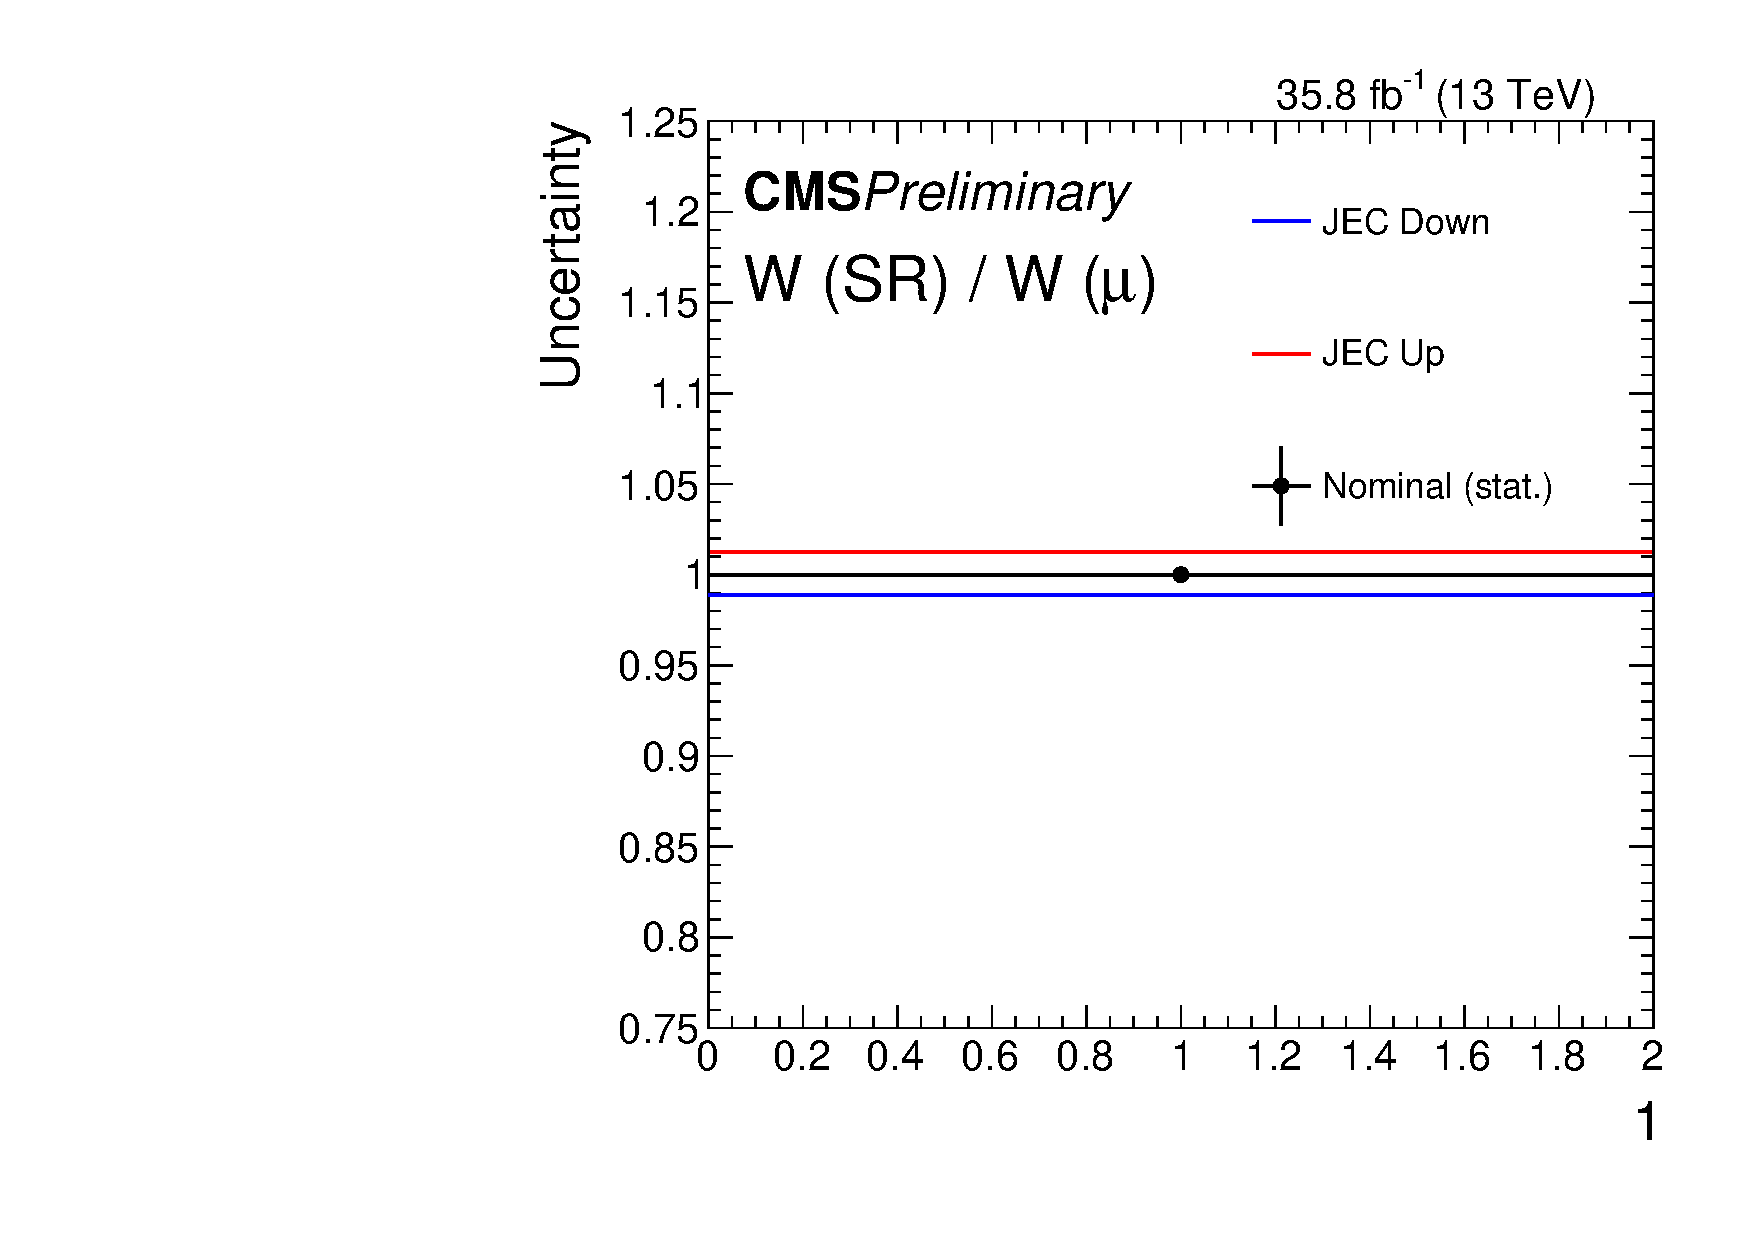
\includegraphics[width=0.45\textwidth]{fig/unc/jec_ratio_WJets_signal_singlemuon_1.pdf}
\caption{{\color{red} Redo for for 2017/18} The resulting jet energy scale uncertainties in the ratios of $W_{SR}/Z_{\nu\nu}$, $Z_{\nu\nu}/Z_{\mu\mu}$ and $W_{SR}/W_{\mu\nu}$, respectively.}
\label{fig:unc_jec}
\end{center}\end{figure}

Lastly, uncertainties in the efficiency of the electron (2\%), and \ptmiss (2\%) triggers, are included and are fully correlated 
across all the bins of dijet mass distribution. 

\begin{table}[htbp]
    \begin{center}
       \begin{tabular}{llc}
       \hline
       \hline
       Source                    & Process                                    & Uncertainty  \\
       \hline
       \hline
       Electron  trigger         & $W_{SR}/W_{e\nu}$, $Z_{\nu\nu}/Z_{ee}$       & 1\% \\
       \MET  trigger             & $W_{SR}/W_{CR}$, $Z_{\nu\nu}/Z_{CR}$, $Z/W$, & 2\% \\
       \hline
       Muon-reco efficiency      & $W_{SR}/W_{\mu\nu}$, $Z_{\nu\nu}/Z_{\mu\mu}$ & 1\% (per leg) \\
       Muon-ID   efficiency      & $W_{SR}/W_{\mu\nu}$, $Z_{\nu\nu}/Z_{\mu\mu}$ & 1\% (per leg) \\
       Muon-Iso   efficiency     & $W_{SR}/W_{\mu\nu}$, $Z_{\nu\nu}/Z_{\mu\mu}$ & 0.5\% (per leg) \\
       Electron-reco efficiency  & $W_{SR}/W_{e\nu}$, $Z_{\nu\nu}/Z_{ee}$       & 1\% (per leg) \\
       Electron-IDiso efficiency & $W_{SR}/W_{e\nu}$, $Z_{\nu\nu}/Z_{ee}$       & 1.5\% (per leg) \\
      \hline
      Lepton veto &  $W_{l,SR}$  & 3\% (QCD), 5.0\% (EW) \\
      \hline
       Jet energy scale         & $W_{CR}/W_{SR}$               & 2\% \\
       Jet energy scale       	& $Z_{CR}/Z_{SR}$				& 1\% \\
       \hline
      \end{tabular}
    \end{center}
    \caption{{\color{red} Check numbers for 2017/18} Summary of experimental uncertainties affecting used in the analysis.}
    \label{tab:systematics}
\end{table}

The remaining uncertainties are for the monte carlo based backgrounds.
A systematic uncertainty of 10\% for the top quark background 
due to the modeling of the top quark \pt distribution in simulation.
The uncertainty in the efficiency of the b jet veto is estimated to be 3\% (1)\% for the top quark (diboson) background. 
In addition, systematic uncertainties of 10 and 20\% are included in the normalizations of the 
top quark~\cite{Khachatryan:2015uqb} and diboson backgrounds~\cite{Khachatryan:2016txa,Khachatryan:2016tgp}, 
respectively, to account for the uncertainties in their cross sections in the relevant 
kinematic phase space. Lastly, the uncertainty in the QCD multijet background estimate
is found to be between 50--150\% due to the variations of the jet response and the
statistical uncertainty of the extrapolation factors. 

\subsection{Control sample validation}

An important cross-check of the application of \pt-dependent NLO QCD and EW corrections
is represented by the agreement between data and simulation in the ratio of 
\Zjets~events and \Wjets~events in the control samples as a function of $m_{jj}$. 

Figure~\ref{fig:Ratio} shows the ratio between \Zmmjets~and \Wmnjets~(left), 
and the one between \Zeejets and \Wenjets~processes (right) as a function of the dijet mass distribution for 
events selected both in multi-bin analysis (top) and single-bin analysis (bottom).
Good agreement is observed between data and simulation after the application of the NLO corrections. 

\begin{figure}[htbp]
  \centering
  \includegraphics[width=0.45\textwidth]{fig/datavalidation/shape/ratio_dimuon_singlemuon_cat_vbf.pdf}
  \includegraphics[width=0.45\textwidth]{fig/datavalidation/shape/ratio_dielectron_singleelectron_cat_vbf.pdf} \\ 
  \includegraphics[width=0.45\textwidth]{fig/datavalidation/shape/ratio_combined_combinedW_cat_vbf.pdf}
  \caption{Comparison between data and MC simulation for, 
     \Zmmjets~and \Wmnjets~(top left), \Zeejets and \Wenjets~processes (top right) ratio  as a function of $m_{jj}$. The combined ratio is shown on bottom.
     The gray bands include both the pre-fit systematic uncertainties and the statistical 
     uncertainty in the simulation. }
  \label{fig:Ratio}
\end{figure}


\subsection{QCD multijet estimation}
{\color{red} Update for 2017/18}
